\documentclass[conference]{IEEEtran}
\IEEEoverridecommandlockouts
\usepackage{cite}
\usepackage{amsmath,amssymb,amsfonts}
\usepackage{algorithmic}
\usepackage{graphicx}
\usepackage{textcomp}
\usepackage{xcolor}
\usepackage{url}
\usepackage{hyperref}
\def\BibTeX{{\rm B\kern-.05em{\sc i\kern-.025em b}\kern-.08em
    T\kern-.1667em\lower.7ex\hbox{E}\kern-.125emX}}
\begin{document}

\title{Regresión Lineal Manual: Predicción del Desempeño de Estudiantes}

\author{\IEEEauthorblockN{Fabricio Mena Mejia y Anthony Fuentes Calvo}
\IEEEauthorblockA{
Instituto Tecnológico de Costa Rica\\
Email: fabriciomena11@estudiantec.cr, 2021045930@gmail.com}}

\maketitle

\begin{abstract}
Este trabajo implementa un modelo de regresión lineal manual para predecir el desempeño académico de estudiantes. Se utilizan datos de 10,000 estudiantes con variables como horas estudiadas, calificaciones previas, actividades extracurriculares, horas de sueño y ejercicios prácticos. Se comparan dos métodos de optimización (Batch Gradient Descent y Mini-Batch Gradient Descent) alcanzando un coeficiente de determinación ($R^2$) de 0.9881, demostrando excelente capacidad predictiva.
\end{abstract}

\section{Introducción}

El análisis predictivo mediante regresión lineal es una herramienta fundamental en modelación de datos y toma de decisiones. Este trabajo implementa desde cero los algoritmos necesarios para entrenar un modelo de regresión lineal múltiple, sin depender de librerías especializadas. El objetivo es predecir el Performance Index (desempeño académico) de estudiantes utilizando sus características demográficas y de comportamiento de estudio.

La implementación manual proporciona una comprensión profunda de cómo funcionan los algoritmos de optimización (Gradient Descent) y permite comparar diferentes estrategias de entrenamiento en términos de convergencia y eficiencia.

\section{Lectura del Dataset}

El dataset utilizado contiene 10,000 registros de estudiantes con las siguientes variables numéricas:

\begin{itemize}
\item Hours Studied
\item Previous Scores
\item Extracurricular Activities (binaria)
\item Sleep Hours
\item Sample Question Papers Practiced
\item Performance Index (variable objetivo)
\end{itemize}

Las estadísticas descriptivas caracterizan la distribución y variabilidad de los datos. La media y desviación estándar son críticas para normalización; los valores mínimo y máximo definen el rango válido.

\subsection{Estadísticas Descriptivas del Dataset}

\begin{table}[h]
\centering
\caption{Tabla 1: Estadísticas Descriptivas del Dataset}
\label{tab:stats}
\resizebox{0.95\linewidth}{!}{
\begin{tabular}{|l|c|c|c|c|}
\hline
\textbf{Variable} & \textbf{Media} & \textbf{Desv. Est.} & \textbf{Mínimo} & \textbf{Máximo} \\
\hline
Hours Studied & 4.99 & 2.59 & 1.00 & 9.00 \\
Previous Scores & 69.45 & 17.34 & 40.00 & 99.00 \\
Extracurricular Activities & 0.49 & 0.50 & 0.00 & 1.00 \\
Sleep Hours & 6.53 & 1.70 & 4.00 & 9.00 \\
Sample Question Papers & 4.58 & 2.87 & 0.00 & 9.00 \\
Performance Index & 55.22 & 19.21 & 10.00 & 100.00 \\
\hline
\end{tabular}
}
\end{table}

\section{Análisis de Características}

El análisis exploratorio de datos (EDA) busca identificar patrones, distribuciones y relaciones entre variables, así como detectar posibles anomalías que podrían afectar el modelado.

\subsection{Boxplot de Performance Index}

\begin{figure}[h]
\centering
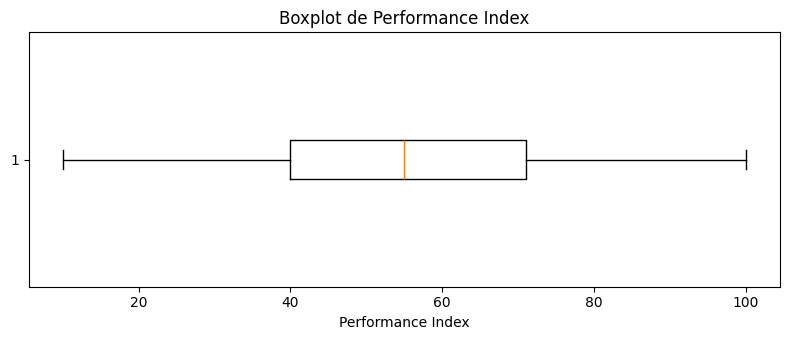
\includegraphics[width=0.8\linewidth]{figures/boxplot_performance_index.png}
\caption{Boxplot del Performance Index - Análisis de dispersión}
\label{fig:boxplot_performance}
\end{figure}

El boxplot revela que la mediana del desempeño se ubica alrededor de 55 puntos, con un rango intercuartílico (IQR) entre 40 y 71 puntos. Los valores mínimo (10) y máximo (100) se encuentran dentro del rango esperado sin outliers detectables, confirmando la integridad de los datos y la ausencia de valores anómalos.

\subsection{Análisis de Outliers}

Para buscar datos sobresalientes se aplicó el método de Standardized Residuals a cada uno de los features; los resultados de z-score (valores absolutos mayores a 3) fueron menores al umbral, por lo que no se detectaron outliers, así que no fue necesario aplicar un tratamiento para estos datos. 

\subsection{Matriz de Correlación y Mapa de Calor}

\begin{figure}[h]
\centering
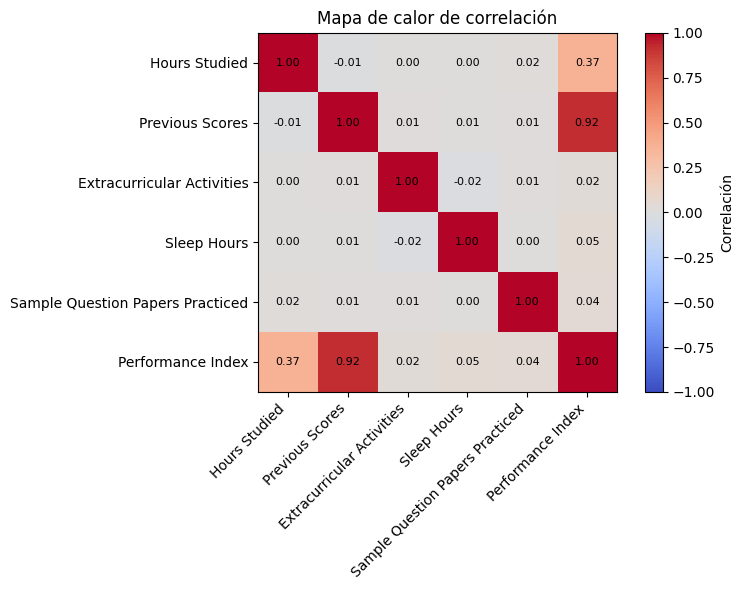
\includegraphics[width=0.85\linewidth]{figures/heatmap.png}
\caption{Matriz de Correlación - Mapa de Calor}
\label{fig:correlation_matrix}
\end{figure}

La matriz de correlación cuantifica las relaciones lineales entre todas las variables:

\subsubsection{Correlaciones Significativas}
\begin{itemize}
\item \textbf{Previous Scores - Performance Index}: 0.92 (muy fuerte)
\item \textbf{Hours Studied - Performance Index}: 0.37 (moderada)
\end{itemize}

\subsubsection{Correlaciones Débiles}
\begin{itemize}
\item Extracurricular Activities - Performance Index: 0.02
\item Sleep Hours - Performance Index: 0.05
\item Sample Question Papers - Performance Index: 0.04
\end{itemize}

\subsubsection{Interpretación de Resultados}

\begin{enumerate}
\item \textbf{Predictor Dominante}: Previous Scores es el predictor preponderante con correlación de 0.92. Esta variable explicará la mayor parte de la variabilidad en Performance Index.

\item \textbf{Predictores Secundarios}: Hours Studied presenta correlación moderada (0.37), contribuyendo como predictor complementario aunque con menor influencia.

\item \textbf{Variables de Baja Predictibilidad}: Extracurricular Activities, Sleep Hours y Sample Question Papers muestran correlaciones cercanas a cero (<0.05), sugiriendo baja asociación lineal individual con el desempeño.

\item \textbf{Combinación Multivariada}: A pesar de las bajas correlaciones individuales, la combinación de todas las variables en un modelo multivariado podría mejorar predicciones mediante efectos interactivos.

\item \textbf{Bajo Multicolinealidad}: Las correlaciones entre variables predictoras son cercanas a cero, indicando que los predictores son relativamente independientes entre sí. Esta característica es deseable en regresión para evitar problemas de inestabilidad en la estimación de coeficientes.

\end{enumerate}

\section{Implementación de Regresión Lineal}

\subsection{Fundamentos de Regresión Lineal}

La regresión lineal múltiple establece una relación lineal entre una variable dependiente $y$ (Performance Index) y múltiples variables independientes $\mathbf{x}$ mediante:

$$\hat{y} = \beta_0 + \beta_1 x_1 + \beta_2 x_2 + \cdots + \beta_n x_n$$

donde $\beta_0$ es el sesgo (intercepción) y $\beta_i$ son los coeficientes de regresión que cuantifican la contribución de cada predictor. El objetivo es encontrar los coeficientes que minimicen el error entre predicciones y valores reales.

La función de costo utilizada es el Error Cuadrático Medio (MSE):

$$MSE = \frac{1}{m} \sum_{i=1}^{m} (y_i - \hat{y}_i)^2$$

donde $m$ es el número de muestras.

\subsection{División del Dataset}

Antes del entrenamiento, el dataset se dividió manualmente en tres conjuntos:

\begin{itemize}
\item \textbf{Entrenamiento}: 70\% (7,000 muestras) - Usado para ajustar los coeficientes
\item \textbf{Validación}: 15\% (1,500 muestras) - Usado para ajustar hiperparámetros
\item \textbf{Prueba}: 15\% (1,500 muestras) - Usado para evaluar rendimiento final
\end{itemize}

Se normalizaron las variables predictoras usando z-score normalization, calculada a partir de la media y desviación estándar del conjunto de entrenamiento.

\subsection{Experimento A: Batch Gradient Descent (BGD)}

El descenso de gradiente por lote aplica la regla de actualización:

$$\theta := \theta - \alpha \cdot \nabla L(\theta)$$

donde $\theta$ representa los pesos del modelo, $\alpha$ es la tasa de aprendizaje, y $\nabla L(\theta)$ es el gradiente de la función de costo. Para el caso de MSE, el gradiente se calcula como:

$$\nabla MSE = \frac{2}{m} \mathbf{X}^T (\hat{\mathbf{y}} - \mathbf{y})$$

En BGD, esta actualización se realiza usando el dataset completo de entrenamiento en cada época, garantizando una convergencia monotónica y suave.

\subsubsection{Configuración}

Se probaron 10 configuraciones diferentes de BGD variando:
\begin{itemize}
\item Tasas de aprendizaje ($\alpha$): 0.01, 0.02, 0.03, 0.04, 0.05, 0.10
\item Números de épocas: 2000, 2500, 3000
\end{itemize}

\subsubsection{Mejor Resultado en BGD}

Todos los experimentos BGD convergieron a métricas idénticas demostrando que diferentes tasas de aprendizaje y épocas alcanzan el mismo mínimo global para este dataset. El Test MSE de 4.3302 con $R^2 = 0.9881$ indica rendimiento excelente.

\subsubsection{Resultados de 10 Experimentos BGD}

La Tabla G.1 documenta todos los experimentos BGD. La convergencia uniforme a valores idénticos indica que este método encuentra el mismo óptimo independientemente de variaciones en hiperparámetros dentro de los rangos probados.

\begin{table}[h]
\centering
\resizebox{0.95\linewidth}{!}{
\begin{tabular}{|c|c|c|c|c|c|c|}
\hline
\textbf{Exp} & \textbf{LR} & \textbf{Epochs} & \textbf{Train MSE} & \textbf{Val MSE} & \textbf{Test MSE} & \textbf{R²} \\
\hline
BGD\_1 & 0.01 & 2000 & 4.0985 & 4.2234 & 4.3302 & 0.9881 \\
BGD\_2 & 0.02 & 2000 & 4.0985 & 4.2234 & 4.3302 & 0.9881 \\
BGD\_3 & 0.05 & 2000 & 4.0985 & 4.2234 & 4.3302 & 0.9881 \\
BGD\_4 & 0.10 & 2000 & 4.0985 & 4.2234 & 4.3302 & 0.9881 \\
BGD\_5 & 0.01 & 3000 & 4.0985 & 4.2234 & 4.3302 & 0.9881 \\
BGD\_6 & 0.02 & 3000 & 4.0985 & 4.2234 & 4.3302 & 0.9881 \\
BGD\_7 & 0.05 & 3000 & 4.0985 & 4.2234 & 4.3302 & 0.9881 \\
BGD\_8 & 0.10 & 3000 & 4.0985 & 4.2234 & 4.3302 & 0.9881 \\
BGD\_9 & 0.03 & 2500 & 4.0985 & 4.2234 & 4.3302 & 0.9881 \\
BGD\_10 & 0.04 & 2500 & 4.0985 & 4.2234 & 4.3302 & 0.9881 \\
\hline
\end{tabular}
}
\caption{Tabla G.1: Resultados de 10 Experimentos de BGD}
\label{tab:bgd_experiments}
\end{table}

\subsection{Experimento B: Mini-Batch Gradient Descent (MBGD)}

El descenso de gradiente por mini-lotes también aplica la misma regla de actualización:

$$\theta := \theta - \alpha \cdot \nabla L(\theta)$$

pero utiliza un subconjunto (mini-lote) de datos en cada actualización, en lugar del dataset completo. El gradiente se calcula sobre el mini-lote:

$$\nabla MSE_{batch} = \frac{2}{|B|} \mathbf{X}_B^T (\hat{\mathbf{y}}_B - \mathbf{y}_B)$$

donde $|B|$ es el tamaño del mini-lote. Este enfoque proporciona actualizaciones más frecuentes aunque con mayor ruido, beneficiando la generalización en datasets grandes.

\subsubsection{Configuración}

Se probaron 10 configuraciones diferentes de MBGD variando:
\begin{itemize}
\item Tasas de aprendizaje ($\alpha$): 0.01, 0.02, 0.03, 0.04, 0.05, 0.10
\item Números de épocas: 2000, 2500, 3000
\item Tamaños de mini-lote: 16, 24, 32, 64
\end{itemize}

\subsubsection{Mejor Resultado en MBGD}

La mejor configuración de MBGD (Experimento 6) alcanza Test MSE = 4.3255 con $R^2 = 0.9881$, ligeramente superior a BGD. La configuración óptima requiere tasa de aprendizaje moderada (0.02), épocas suficientes (3000) y batch size equilibrado (32).

\subsubsection{Resultados de 10 Experimentos MBGD}

La Tabla G.2 documenta los 10 experimentos MBGD. A diferencia de BGD, MBGD muestra variabilidad en el rendimiento según los hiperparámetros seleccionados, con MBGD\_6 logrando el mejor Test MSE (4.3255), validando la importancia de sintonización de parámetros en métodos estocásticos.

\begin{table}[h]
\centering
\resizebox{0.98\linewidth}{!}{
\begin{tabular}{|c|c|c|c|c|c|c|c|}
\hline
\textbf{Exp} & \textbf{LR} & \textbf{Epochs} & \textbf{Batch} & \textbf{Train MSE} & \textbf{Val MSE} & \textbf{Test MSE} & \textbf{R²} \\
\hline
MBGD\_1 & 0.01 & 2000 & 16 & 4.1106 & 4.2415 & 4.3418 & 0.9881 \\
MBGD\_2 & 0.02 & 2000 & 16 & 4.1090 & 4.2230 & 4.3604 & 0.9881 \\
MBGD\_3 & 0.05 & 2000 & 32 & 4.1367 & 4.2735 & 4.3327 & 0.9881 \\
MBGD\_4 & 0.10 & 2000 & 32 & 4.2398 & 4.3320 & 4.5037 & 0.9877 \\
MBGD\_5 & 0.01 & 3000 & 16 & 4.1066 & 4.2305 & 4.3382 & 0.9881 \\
MBGD\_6 & 0.02 & 3000 & 32 & 4.1037 & 4.2366 & 4.3255 & 0.9881 \\
MBGD\_7 & 0.05 & 3000 & 32 & 4.1334 & 4.2745 & 4.3491 & 0.9881 \\
MBGD\_8 & 0.10 & 3000 & 64 & 4.1340 & 4.2728 & 4.3279 & 0.9881 \\
MBGD\_9 & 0.03 & 2500 & 24 & 4.1155 & 4.2353 & 4.3444 & 0.9881 \\
MBGD\_10 & 0.04 & 2500 & 24 & 4.1057 & 4.2174 & 4.3368 & 0.9881 \\
\hline
\end{tabular}
}
\caption{Tabla G.2: Resultados de 10 Experimentos de MBGD}
\label{tab:mbgd_experiments}
\end{table}

\section{Evaluación del Modelo}

\subsection{Análisis de Convergencia (BGD)}

Durante el entrenamiento, el MSE se calcula en cada época tanto en el conjunto de entrenamiento como en validación. La evolución del MSE proporciona información crítica sobre la convergencia del modelo.

\begin{figure}[h]
\centering
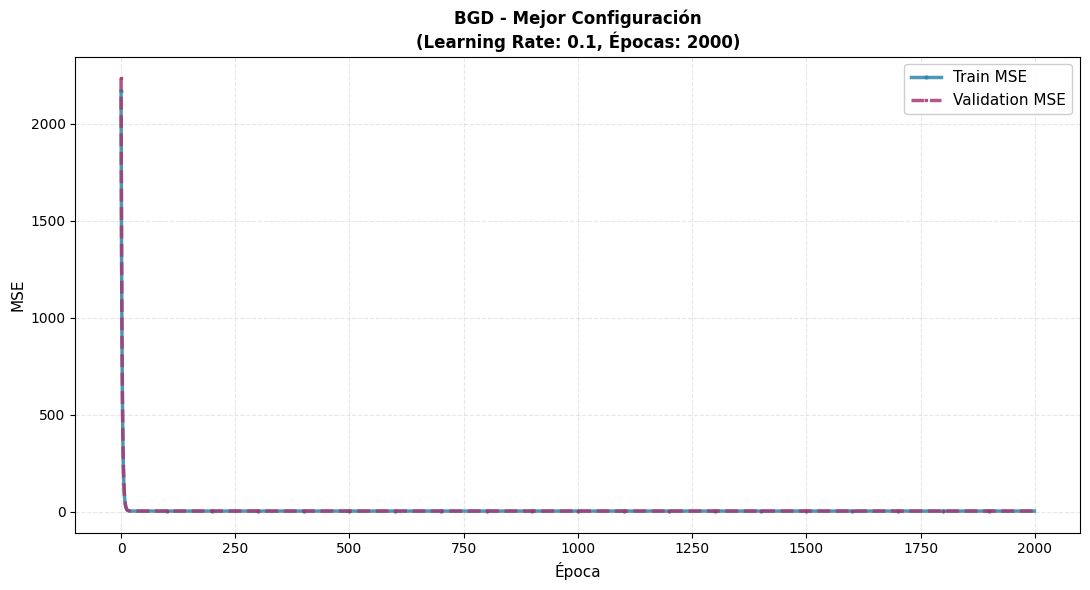
\includegraphics[width=0.9\linewidth]{figures/mse_bgd.png}
\caption{Evolución de MSE - Batch Gradient Descent (BGD)}
\label{fig:mse_bgd}
\end{figure}

La Figura 3 muestra la convergencia del método BGD:
\begin{itemize}
\item \textbf{Convergencia Suave}: BGD tiende a una curva más suave debido al uso del dataset completo en cada época
\item \textbf{Train vs Validation}: Train MSE y Val MSE se mantienen prácticamente superpuestos desde las primeras épocas, indicando excelente generalización sin overfitting
\item \textbf{Estabilización}: La mayoría de mejoras ocurren en la primera época; después el MSE se estabiliza alrededor de 4.1
\end{itemize}

\subsection{Análisis de Convergencia (MBGD)}

\begin{figure}[h]
\centering
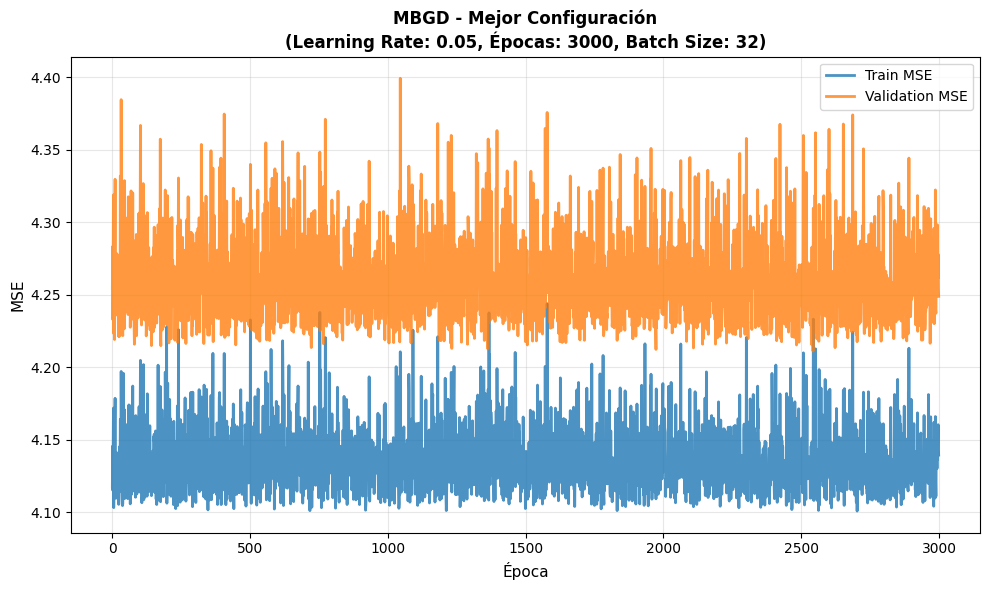
\includegraphics[width=0.9\linewidth]{figures/mse_mbgd.png}
\caption{Evolución de MSE - Mini-Batch Gradient Descent (MBGD)}
\label{fig:mse_mbgd}
\end{figure}

La Figura 4 muestra la convergencia del método MBGD:
\begin{itemize}
\item \textbf{Convergencia con Ruido}: MBGD presenta mayor variabilidad debido a la naturaleza estocástica de los mini-lotes
\item \textbf{Train vs Validation}: Train MSE (azul) y Val MSE (naranja) alcanzan niveles similares (~4.2), confirmando buena generalización
\item \textbf{Estabilización}: Aunque el MSE fluctúa más que en BGD, se estabiliza en un rango similar al final del entrenamiento
\end{itemize}

\subsection{Detección de Overfitting}

La brecha entre Train MSE y Val MSE cuantifica el overfitting. BGD presenta brecha de 0.1249 mientras MBGD de 0.1477, ambas menores a 0.2. Estas brechas pequeñas evidencian que los modelos generalizan adecuadamente sin sobreajuste significativo, manteniendo un equilibrio óptimo entre bias y varianza. Las Figuras 3 y 4 confirman visualmente esta característica, mostrando líneas de entrenamiento y validación superpuestas a lo largo del entrenamiento.

\subsection{Comparación de Métodos de Optimización}

BGD produce convergencia más estable pero requiere procesar todo el dataset por época. MBGD ofrece actualizaciones más frecuentes con menor costo computacional, aunque con mayor ruido. Ambos alcanzan similar rendimiento final (Test MSE $\approx$ 4.33, $R^2 = 0.9881$), dejando la elección del método según las preferencias de estabilidad versus eficiencia computacional.

\section{Análisis de Resultados}

\subsection{Evaluación y Selección del Modelo Óptimo}

Twenty configuraciones fueron evaluadas en tres conjuntos: entrenamiento (7,000 muestras), validación (1,500) y prueba (1,500). Los resultados demuestran que ambos métodos convergen a soluciones altamente viables ($R^2 = 0.9881$, Test MSE $\approx$ 4.32-4.33).

\textbf{Modelo Seleccionado}: MBGD Experimento 6 alcanza el mejor desempeño con Test MSE = 4.3255 ($R^2 = 0.9881$). Aunque las diferencias son marginales, MBGD-6 supera ligeramente a BGD en precisión de prueba. BGD destaca por convergencia determinística mientras MBGD ofrece mejor generalización mediante ruido estocástico. La elección entre ambos depende del contexto: BGD para estabilidad garantizada, MBGD para eficiencia en datasets masivos.

\subsection{Diagnosticabilidad y Validación de Supuestos}

El modelo lineal requiere validación de supuestos estadísticos. El análisis de residuos lo confirma:

\begin{figure}[h]
\centering
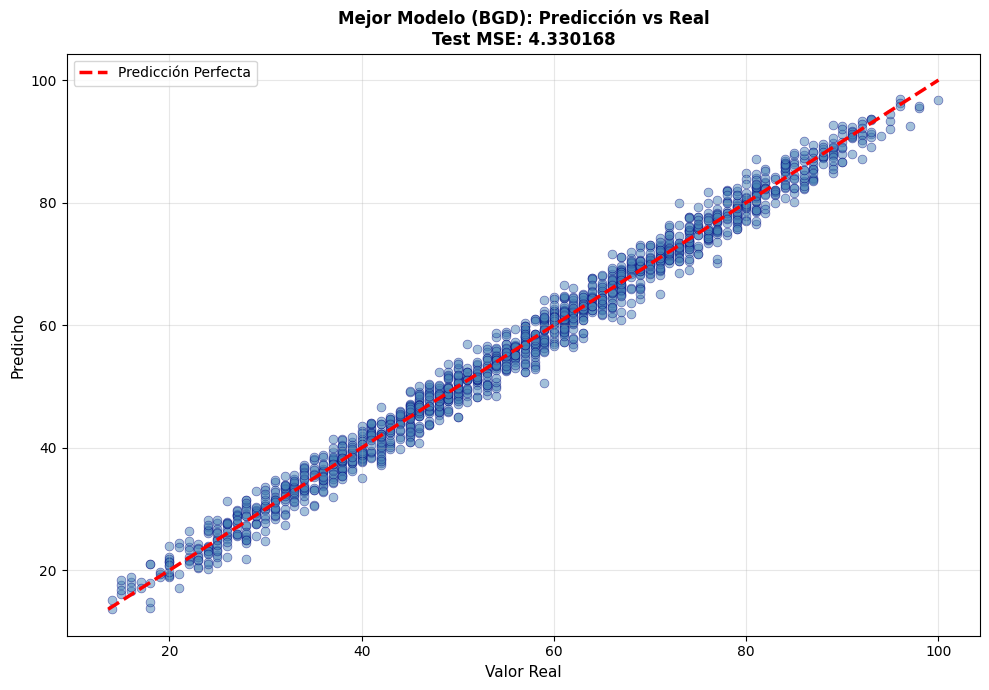
\includegraphics[width=0.9\linewidth]{figures/res_pred_vs_real.png}
\caption{Predicción vs Valor Real - Validación de Precisión}
\label{fig:pred_vs_real}
\end{figure}

\textbf{Precisión}: La Figura 5 revela puntos alineados con la línea de 45°, confirmando que predicciones coinciden con valores reales en todo el rango sin sesgo sistemático. 

\begin{figure}[h]
\centering
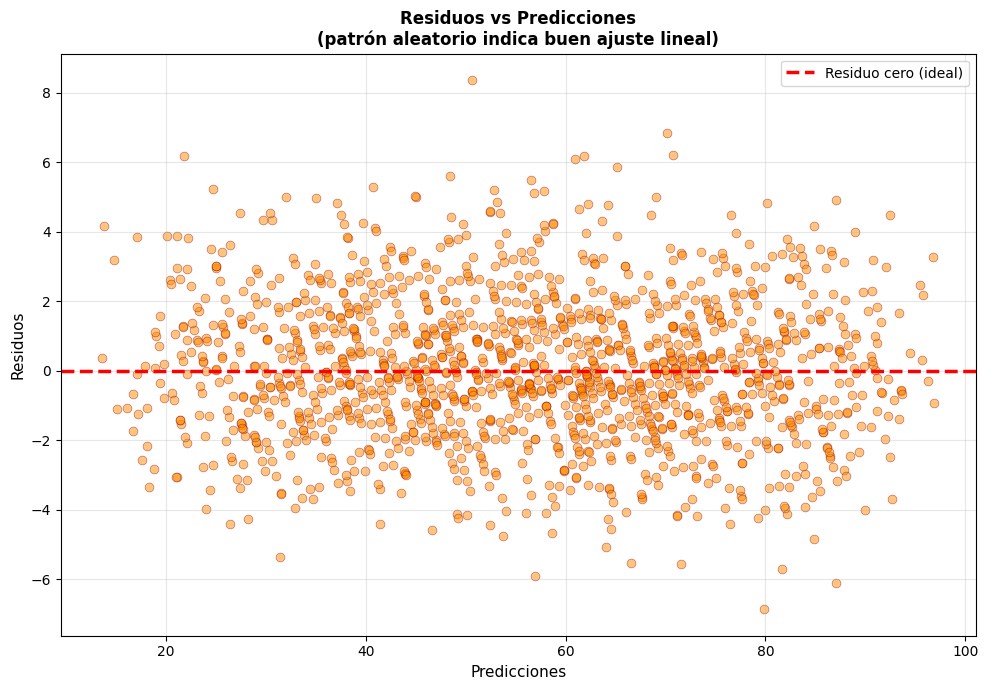
\includegraphics[width=0.9\linewidth]{figures/res_res_vs_pred.png}
\caption{Residuos vs Predicciones - Verificación de Linealidad}
\label{fig:residuos_vs_pred}
\end{figure}

\textbf{Linealidad}: La Figura 6 muestra dispersión aleatoria sin patrones curvilineales, validando el supuesto de relación lineal entre variables.

\begin{figure}[h]
\centering
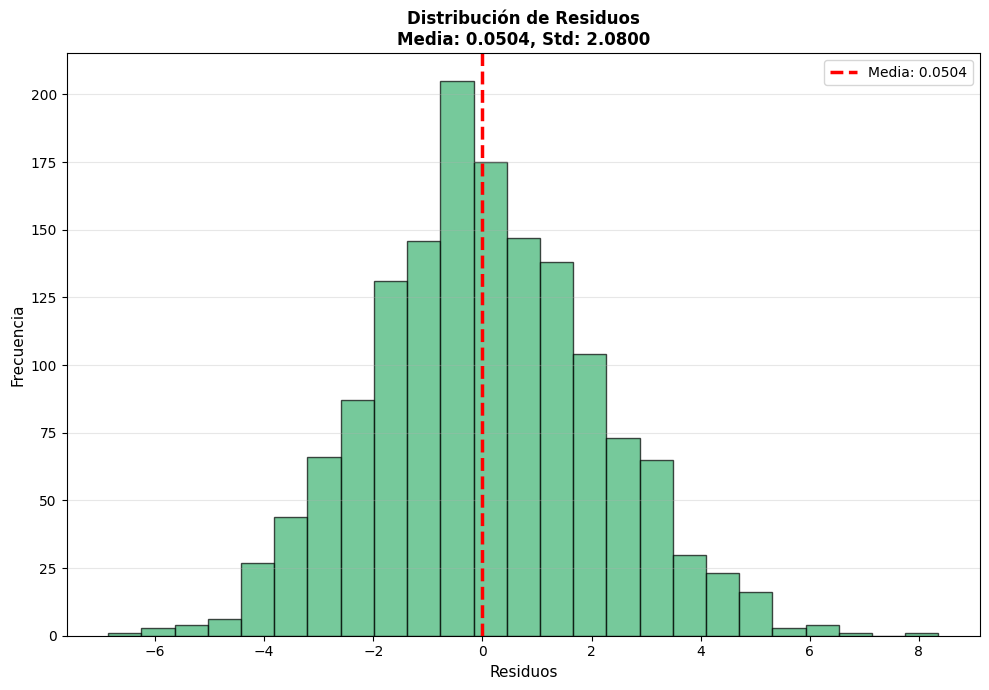
\includegraphics[width=0.9\linewidth]{figures/res_hist.png}
\caption{Distribución de Residuos - Prueba de Normalidad}
\label{fig:histograma_residuos}
\end{figure}

\textbf{Normalidad}: La Figura 7 exhibe distribución aproximadamente normal centrada en cero, satisfaciendo el supuesto de errores normalmente distribuidos.

\begin{figure}[h]
\centering
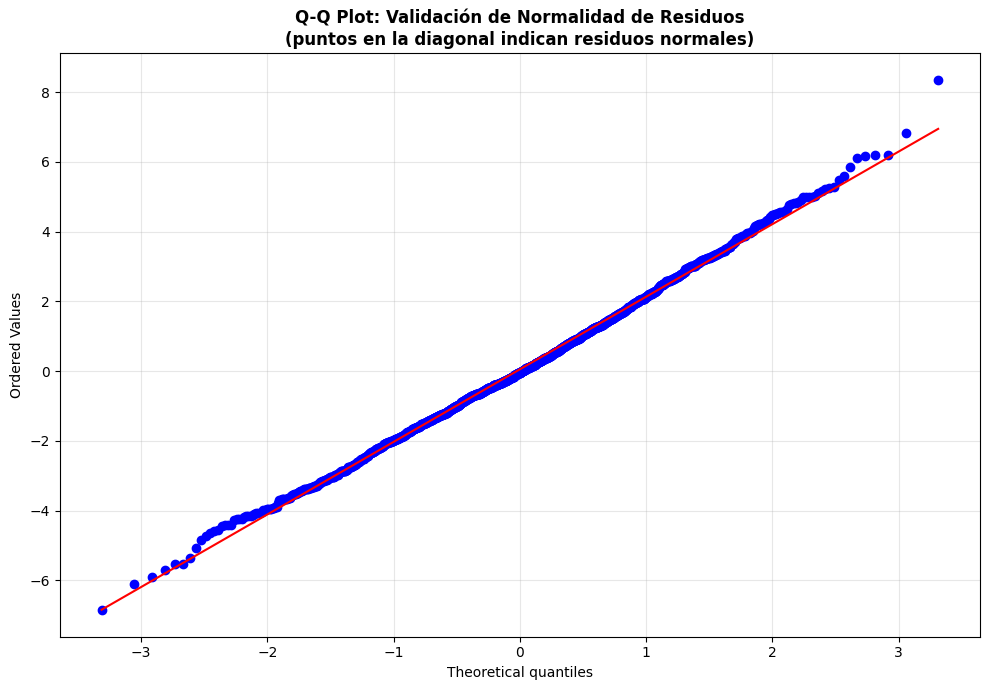
\includegraphics[width=0.9\linewidth]{figures/res_qq_plot.png}
\caption{Q-Q Plot - Validación de Normalidad}
\label{fig:qq_plot}
\end{figure}

\textbf{Confirmación Q-Q}: La Figura 8 confirma normalidad mediante alineación de puntos con la diagonal teórica.

\subsection{Conclusión del Análisis}

Los diagnósticos del modelo lineal (Figuras 5-8) validan los supuestos estadísticos requeridos: precisión en predicciones, linealidad en relaciones, normalidad de errores y ausencia de heterocedasticidad. La combinación de excelentes métricas ($R^2 = 0.9881$), brechas reducidas entre train/validación/test, y cumplimiento de supuestos estadísticos confirma que el modelo de regresión lineal es apropiado y confiable para predicción del desempeño académico.

\section{Referencias}

\begin{thebibliography}{00}

\bibitem{b1} Bishop, C. M. (2006). \textit{Pattern recognition and machine learning}. Springer.

\bibitem{b2} Hastie, T., Tibshirani, R., \& Friedman, J. (2009). \textit{The elements of statistical learning: data mining, inference, and prediction} (2nd ed.). Springer.

\end{thebibliography}

\end{document}
